\begin{questions} 

% \question[3] This is a multiple choice question
% \begin{choices}
%    \choice \chooseone
%    \choice \chooseone
%    \choice \chooseone
%    \choice \chooseone
%    \choice \chooseone None of the above.
% \end{choices}



\question[3]  Find an equation for the line which is perpendicular to and has the same $y$-intercept as the line $y=-2x+\frac{1}{3}$
\begin{choices}
   \choice \chooseone $y=2x+\frac{1}{3}$
   \choice \chooseone $y=-2x-3$
   \choice \chooseone $y=\frac{1}{2}x-3$
   \choice \chooseone $y=\frac{1}{2}x+\frac{1}{3}$
   \choice \chooseone None of the above.
\end{choices}

\vfill

\question[3] %(Joey) 
 \textbf{Select ALL} of the following that are functions:% relations:
\begin{multicols}{2}
\checkboxchar{\Large$\Box$}\begin{checkboxes}

\choice \phantom{a}\vspace{-.7cm}

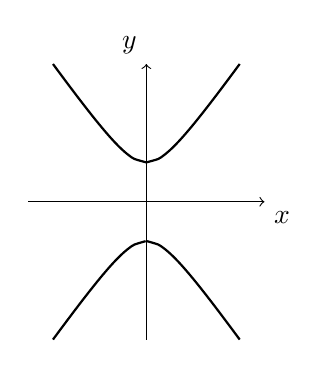
\begin{tikzpicture}[scale=.5]
    % Draw axes
    \draw[->] (-3, 0) -- (3, 0) node[anchor=north west] {$x$};
    \draw[->] (0, -3.5) -- (0, 3.5) node[anchor=south east] {$y$};
    

    
    % Draw the hyperbola branches (now vertically oriented)
    \draw[thick, smooth, domain=1:3.5, samples=30] plot ({sqrt((\x)^2/2 - .5)}, \x);
    \draw[thick, smooth, domain=1:3.5, samples=30] plot ({-sqrt((\x)^2/2 - .5)}, \x);
    \draw[thick, smooth, domain=-3.5:-1, samples=30] plot ({sqrt((\x)^2/2 - .5)}, \x);
    \draw[thick, smooth, domain=-3.5:-1, samples=30] plot ({-sqrt((\x)^2/2 - .5)}, \x);
    

\end{tikzpicture}
\vspace{1cm}
\choice \phantom{a}\vspace{-.7cm}

\hspace{1cm}
\begin{tabular}{|l|l|}
\hline $x$ & $y$ \\\hline
\hline $\pi$ & Pi \\
\hline $\xi$ & Xi \\
\hline $\zeta$ & Zeta \\
\hline $\varpi$ & Pi \\
\hline
\end{tabular}
\vfill
\choice \phantom{a}\vspace{-.7cm}

  \begin{tikzpicture}
    \foreach[count=\i] \lseti/\lsetmi in {A/{x,y,z,w},B/{a,b,c}} {
        \begin{scope}[local bounding box=\lseti, x=3cm, y=.5cm]
        \foreach[count=\j] \lj in \lsetmi {
            \node[minimum width=1em] (n-\j-\lseti) at (\i,-\j) {\lj};
        }
        \end{scope}
        \node[ellipse, draw, fit=(\lseti), 
        label={[name=l-\lseti]above:$\lseti$}] {};
    }
    \draw[->] (n-1-A) -- (n-2-B);
    \draw[->] (n-2-A) -- (n-1-B);
   % \draw[->] (n-3-A) -- (n-1-B);
    \draw[->] (n-3-A) -- (n-3-B);
    \draw[->] (n-4-A) -- (n-3-B);
\end{tikzpicture}
\vspace{1cm}
\choice
\phantom{a}\vspace{-.7cm}
    
    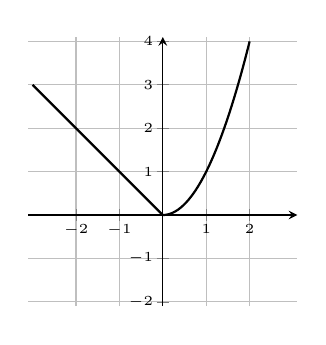
\begin{tikzpicture}%[domain=-4:4]
    \begin{axis}[
    grid=major,
    axis x line = middle,
    axis y line = middle,
        yticklabel style = {font=\tiny,xshift=0.5ex},
        xticklabel style = {font=\tiny,yshift=0.5ex},
    %scale only axis=true,
    width=5 cm,
    height=5 cm,
    xtick={-2,-1,0,1,2},
    ytick={-2,-1,0,1,2,3,4},
    xmin=-3.1,
    xmax=3.1,
    ymin=-2.1,
    ymax=4.1,
    ]
\addplot[smooth, thick, domain = 0:2,samples=35] { (x^2)};
\addplot[smooth, thick, domain = -3:0,samples=35] { -x};
  \end{axis}
\end{tikzpicture}
\end{checkboxes}
\end{multicols}
\vfill

\question[3] \textbf{Select ALL} (real and complex) solutions to the equation: \[x^4-1=0 \]
    \checkboxchar{\Large$\Box$}\begin{checkboxes}
        \choice $x=0$
        \choice $x=1$
        \choice $x=-1$
        \choice $x=i$   
        \choice $x=-i$
    \end{checkboxes}
%\vfill

\newpage
    \question[3] Find the domain of the function:
\[ \dfrac{\sqrt{x+5}}{x-4}\]
\begin{choices}
    \choice \chooseone $(-\infty, -5)\bigcup(-5,4)\bigcup(4,\infty)$
    \choice \chooseone $(-\infty, 4)\bigcup(4,\infty)$
    \choice \chooseone $[-5,4)\bigcup(4,\infty)$
    \choice \chooseone $(-\infty, -5]\bigcup[5,\infty)$
    \choice \chooseone None of the Above.
\end{choices}



\question[3] Find the solution to the following inequality
\[|x-2|\le-2\]
\begin{choices}
   \choice \chooseone $(-\infty,\infty)$
   \choice \chooseone $(-\infty,0]\cup[4,\infty)$
   \choice \chooseone There is no $x$ that solves the inequality.
   \choice \chooseone $[0,4]$
\end{choices}

\question[3] Gilbert is solving a quadratic using completing the square. He has isolated the $x$-terms on one side of the equation to find:
\[x^2-6x=2\]
What does he \underline{add to both sides} of the equation in the next step of completing the square?
\begin{choices}
    \choice \chooseone 3
    \choice \chooseone 9
    \choice \chooseone $-9$
    \choice \chooseone $-2$
    \choice \chooseone None of the above.
\end{choices}

\newpage
\hspace{-.5in}Free answer section. Work must be shown to get credit for any answer. Partial credit may be given even for incorrect final answers, so show your work.

\question[7] Evaluate the following. (In your final answer, make sure that the numerator and the denominator do not contain a common factor other than 1.)
    % \begin{parts}
     \vspace{.5cm}
     
    % 	\part[5] 
     $\displaystyle{\frac{x+2}{x^2+4x+3}+\frac{x+3}{2x+2}}$
        \vfill
%    	\part[5] $\displaystyle{\left(\frac{x+2}{x^2+4x+3}\right) \cdot \left(\frac{x+3}{2x+2}\right)}$
        \vfill
    % \end{parts}

%\newpage

\question[6] Factor the following quadratic. 
% \begin{parts}
%      \part[5] 
     $5 x^2+14 x-3$
      \vfill
     % \part[5] $x^2+14 x+49$
     % \vfill

%\end{parts}

    

\newpage

\question[7] Solve for $x$:
    \[ x^2 + 10x +50 = 1-4x\]
    \vfill%\vfill

\question[7] Solve for $x$:
    \[ x^2+2x-9=0 \]
    \vfill

\newpage

\question[5] Consider the points $A=(1,1)$ and $B=(4,3)$.

% \begin{parts}
%     	\part 
     Find an equation for the line passing through the points $A$ and $B$. Give your answer in point-slope form.
        \vfill

        % \vfill
    % \end{parts}


%Jenny absolute value
\question[7] Solve the following inequality (Give your answer in interval notation):
% \vspace{0.5cm}
% \begin{parts}
%     \part 
    \[|6-3x|-2\geq 7\]
    \vspace{9cm}
    % \part  
    % $|x-2|+5<3$
  % \vspace{13cm}
% \end{parts}

\newpage %Solving nonlinear equations by Lizhe

 \question[6] 
% Solve the following equations.

% \begin{parts}
%     \part[6] 
    Find \textbf{all} solutions to the following equation: 
%    (Note: Solutions may be real or complex)
    \[ x^4 -11x^2  +18= 0.\]
        \vfill
    % \part[5] Find all solutions to the following equation:
    %  \[ x^3 -3x^2  = 10x.\]
    %  %(Hint: You may use your result in part (a).)
    %     \vfill
    % \end{parts}
    

%\newpage

%Yuchen Inequalities

\question Solve each of the following inequalities. For each part, express your answer in interval notation.% and then graph it on a number line.}
\begin{parts}
    % \part[5] $8\le-2x+3$
    % \vspace{5cm}
    \part[5] $-9\le4-5x<6$
    \vfill%\vspace{5cm}
    \part[7] $-2x^2\ge-7x+6$
    \vfill\vfill%\vspace{5cm}
\end{parts}
\newpage


\question[6] Draw a graph of the following function, for $-5 \le x \le 5$:

\[
f(x) = \begin{cases}
x-1 & x < 0 \\
-x & 0 \le x \le 2 \\
-2 & 2 < x \\
\end{cases}
\]



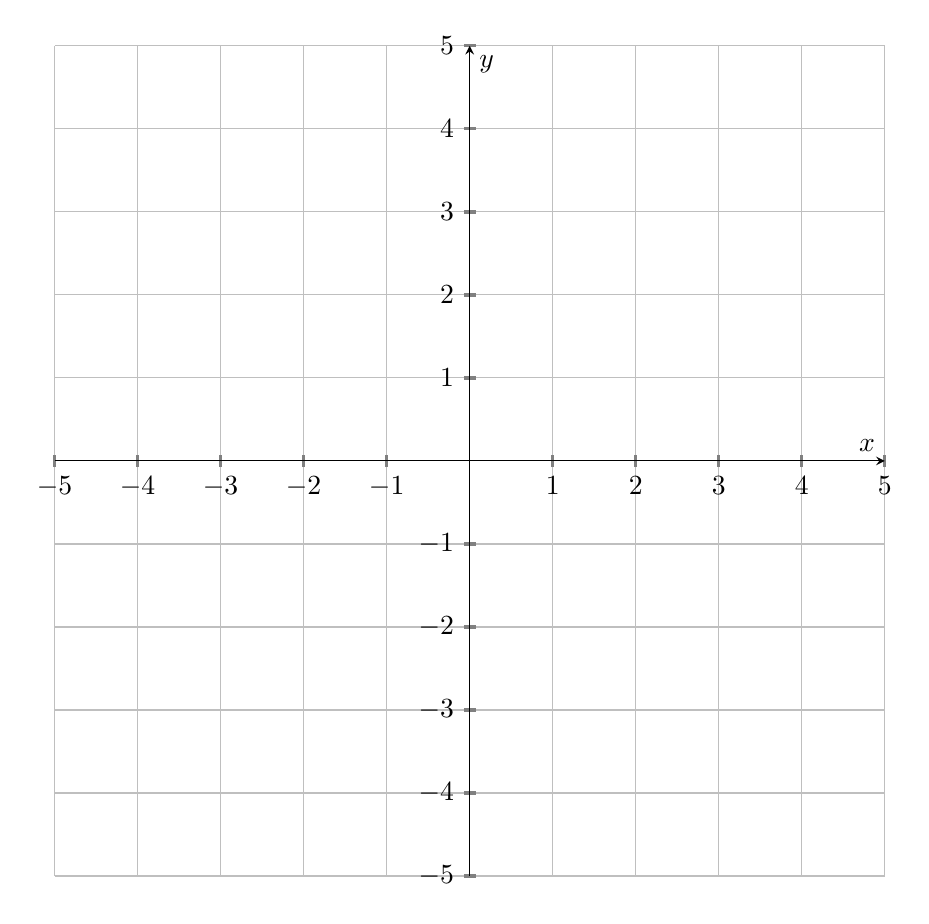
\begin{tikzpicture}
\begin{axis}[
  width= \textwidth,
  height= \textwidth,
  axis lines=middle,
  grid=major,
  xmin=-5,
  xmax=5,
  ymin=-5,
  ymax=5,
  xlabel=$x$,
  ylabel=$y$,
  xtick={-5,-4,...,5},
  ytick={-5,-4,...,5},
  tick style={very thick},
  legend style={
  at={(rel axis cs:0,1)},
  anchor=north west,draw=none,inner sep=0pt,fill=gray!10}
]
\end{axis}
\end{tikzpicture}


\newpage

\question Below is a graph of the water temperatures of Lake Mendota ($f(x)$, curved, solid line) and Lake Michigan ($g(x)$, pointy, dashed line) over the course of one year.
\begin{center}
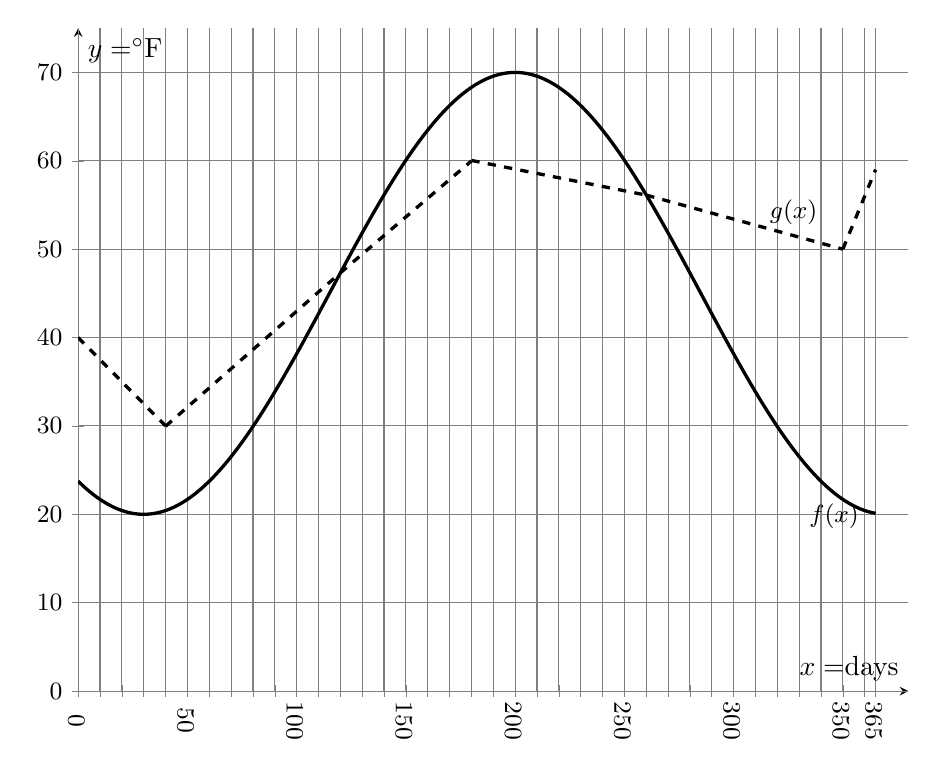
\begin{tikzpicture}[scale = 1]
    \begin{axis}[
        domain=0:365, % Defines the x range
        samples=200,  % Number of samples for smoothness
        width = \textwidth,
        height = 10cm,
        xlabel={$x=$days},
        ylabel={$y= ^\circ$F},
        axis lines=middle,
        grid=major, % Show only the main grid by default
        major grid style={solid, gray}, % Style for the main grid lines
        minor grid style={solid, lightgray}, % Style for the subgrid (lighter grey)
        xmin=0, xmax=380,  % Sets x-axis range
        ymin=0, ymax=75,  % Sets y-axis range
        xtick={0, 50, 100, 150, 200, 250, 300, 350, 365}, % Main ticks for x-axis
        ytick={0, 10, 20, 30, 40, 50, 60, 70}, % Main ticks for y-axis
        extra y ticks = {0},
        extra x ticks={0, 10,20,...,360}, % Subgrid ticks for x-axis
        extra x tick labels={0}, % Suppress labels for x subgrid ticks
        extra y tick labels={0}, % Suppress labels for y subgrid ticks
        legend pos=north east,
        tick label style={font=\small}, % Make the tick labels smaller
        xticklabel style={rotate=270, anchor= south, xshift=.3cm, yshift = -.25cm} % Rotate x-axis labels by 270 degrees and shift them down
        ]
    % Plot the sinusoidal function in blue and label as f(x)
    \addplot[very thick]%, blue] 
        {25*sin(deg(pi/170*(x-115))) + 45}
        node[pos=0.95, below] {\small $f(x)$}; % Label the function on the line
    
    % Plot the piecewise function in red and label as g(x)
    \addplot[domain=0:40, very thick, dashed] {-0.25*(x-40) + 30};
    \addplot[domain=40:120, very thick, dashed] {0.217*x + 21.281};
    \addplot[domain=120:180, very thick, dashed] {0.211*x + 22.001};
    \addplot[domain=180:260, very thick, dashed] {-0.049*x + 68.859};
    \addplot[domain=260:350, very thick, dashed] {-0.068*x + 73.8}
    node[pos=0.75, above] {\small $g(x)$};
    \addplot[domain=350:365, very thick, dashed] {.6*(x-350) + 50};
    
    \end{axis}
\end{tikzpicture}
    
\end{center}

\begin{parts}
    %\part[2] What is the domain of $f$?
    %\vspace{1cm}

    \part[2] What is the \underline{range} of $g$?
     \vspace{1cm}
    \part[3] What are the interval(s) where the temperature of Lake Mendota ($f(x)$) is decreasing?
     \vspace{2cm}

    \part[2] \textbf{Identify all} local minima of $g(x)$. %(Fill in all that are minima)
    \checkboxchar{\Large$\Box$}\begin{checkboxes}
    \begin{multicols}{2}
        \choice (40, 30)
        \choice (130, 49)
        \choice (180, 60)
        \choice (210, 10)
        \choice (350, 50)
    \end{multicols}
      
    \end{checkboxes}

    \part[2] What days ($x$ values) do the two lakes have the same temperature (i.e. for what $x$ is $f(x) = g(x)$)
    \vspace{1.5cm}

    %\part[2]  What are the interval(s) when Lake Mendota is warmer than Lake Michigan (i.e. when is $f(x) > g(x)$)?
    
    
\end{parts}
\newpage

\question Find the average rate of change for functions below on indicated intervals.

\begin{parts}
    	\part[7] $f(x) = \dfrac{x^2}{2\sqrt{x + 6}}$ on $[-5,10]$
        \vfill

        \part[3] Below is the graph of a function $g$. Of the three choices below, choose the interval where $g(x)$ has the \underline{largest average rate of change}.

        \begin{multicols}{2}
             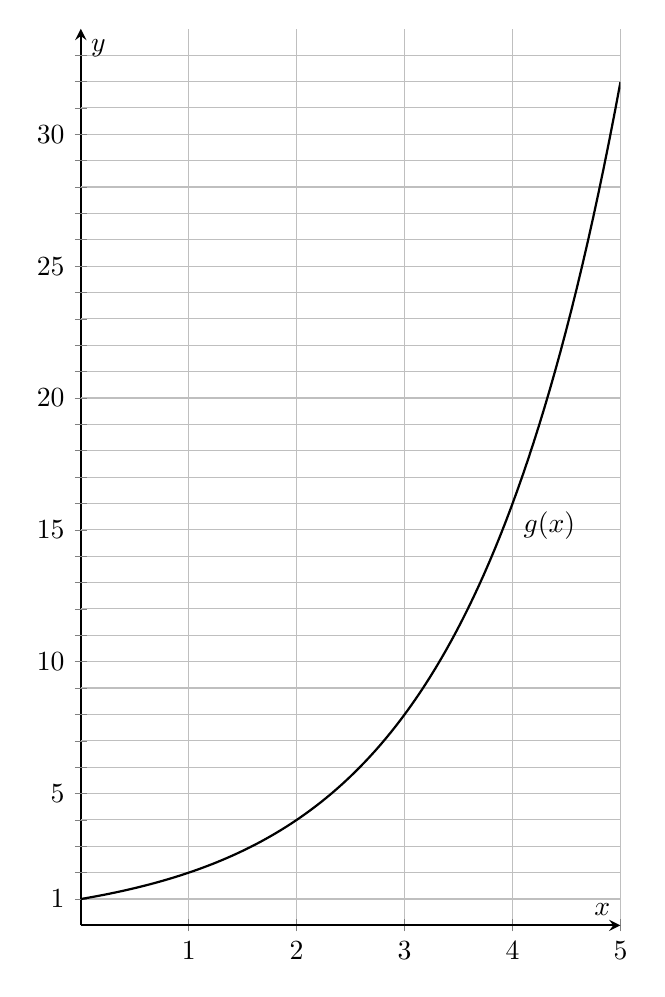
\begin{tikzpicture}
    \begin{axis}[
        % Axis settings
        xlabel={$x$}, ylabel={$y$},
        grid=major, 
        axis lines=middle, 
        % Add a grid
        xmin=0, xmax=5,                  % Set x-axis limits
        ymin=0, ymax=34,                 % Set y-axis limits
        xtick={0,1,2,3, 4, 5},               % Set x-axis tick marks
        extra y ticks = {1, 2, 3,4,5,6,7,8,9,10,11,12,13,14,15,16,17,18,19,20,21,22,23,24,25,26,27,28,29,30,31, 32, 33},
        extra y tick labels={ 1},
         % Set y-axis tick marks
        domain=0:5,                      % Function domain
        samples=100,                     % Number of sample points for smooth curve
        thick,% Line thickness for the plot
        %axis equal
        y post scale=2
    ]

    % Plot the function y = 2^x
    \addplot[black] {2^x}
    node[pos=0.5, below right] {$g(x)$};

    \end{axis}
\end{tikzpicture}
\vspace{2cm}
\checkboxchar{\chooseone}
\begin{checkboxes}
    \choice $[0,3]$
\vfill
    \choice $[3,5]$
\vfill
    \choice $[0,5]$
\end{checkboxes}

\vspace*{4cm}
        \end{multicols}
       
    \end{parts}
\end{questions}